This section describes the detailed implementation of SONIC in \CMSSW; the server used to serve models, NVIDIA Triton Inference Server; and the benefits of running inference with SONIC.

\subsection{Past Studies of SONIC}
\textcolor{red}{This section can probably be shortened and merged into the later section.}

The SONIC approach~\cite{SONIC_origin, SONIC_cms} was introduced in the first notable use of the IaaS scheme in HEP, which employed FPGA coprocessors to accelerate ML algorithms~\cite{Duarte:2019fta}. In this application, the ResNet-50 convolutional neural network~\cite{ResNet50} was retrained as a top quark jet tagger and as a neutrino event classifier. These algorithms were then hosted on the Microsoft Brainwave service~\cite{Brainwave}. It was shown that IaaS enabled per-inference latency reductions by a factor of more than 30, even including overhead and data transfer time between client jobs at Fermilab in Illinois and the Microsoft data center in Virginia.

This work was then extended to study the use of GPUs as coprocessors for multiple LHC-specific applications in Ref.~\cite{Krupa:2020bwg}. There, SONIC was used to enable acceleration of three algorithms:
\begin{enumerate}
    \item A ResNet-50 based top quark jet tagger;
    \item Fast Calorimeter Learning (FACILE), which is a deep neural network for CMS hadron calorimeter (HCAL) energy regression;
    \item DeepCalo, which is a convolutional neural network for electron and photon energy regression in the ATLAS electromagnetic calorimeter~\cite{deepcalo}.
\end{enumerate}
These algorithms represent a wide range of algorithmic complexity and input data size, and all of them show significant speed improvements when running via SONIC. While these algorithms provided an interesting and useful testbed, currently they are not run by default in either the ATLAS or CMS data-processing workflows.

The initial FPGA-based demonstration was similarly extended to a detailed study of GPU-based acceleration in the neutrino experiment context in Ref.~\cite{Wang:2020fjr}. There, the track and particle shower hit identification components of the ProtoDUNE-SP reconstruction chain~\cite{DUNE:2020cqd} were accelerated by a factor of 17. This lead to a 2.7 times reduction in the total processing time per event compared to a CPU-only architecture. In this application, a single GPU could be used to service 68 CPU threads, which is an important demonstration of the flexibility to optimize the CPU-coprocessor ratios in the IaaS paradigm.

Heterogeneous computing frameworks using GPUs have appeared in multiple non-IaaS contexts in HEP recently as well. One of the first significant real-time applications was in the ALICE high-level trigger system~\cite{ALICE:2018phe}, where GPUs were used to accelerate online tracking. Similarly, a fully GPU-based implementation of the first level trigger has been planned for LHCb~\cite{Aaij:2019zbu}, which could be run on about 500 GPUs. For a further overview of GPU usage in real-time applications for HEP, please see Ref.~\cite{VomBruch:2020plx}.

In the CMS context, an algorithm that could accelerate tracking on GPUs with a parallelized cellular automaton approach was introduced in Ref.~\cite{Funke:2014dga}. Using a GPU-enabled heterogeneous architecture in the first layer of the CMS trigger for track triggering was then proposed in Ref.~\cite{Pantaleo:2016ery}, and a GPU-specific version of tracking called ``Patatrack'' has been developed which allows more complex tracking to be performed in triggering stages of data analysis~\cite{Bocci:2020pmi}. The authors of this algorithm proposed a mechanism for \CMSSW jobs to directly interact with local co-processor resources~\cite{Bocci:2020olh}. Similarly, the use of GPU and FPGA resources was investigated to take advantage of the inherent parallelizability of local reconstruction algorithms for the CMS Electromagnetic and Hadronic calorimeters~\cite{Massironi_2020}.%and the use of GPU and FPGA resources was investigated to take advantage of the inherent parallelizability of local reconstruction algorithms for the CMS Electromagnetic and Hadronic calorimeters~\cite{Massironi_2020}. More recently, a GPU-specific version of tracking called ``Patatrack'' has been developed which allows more complex tracking to be performed in triggering stages of data analysis~\cite{Bocci:2020pmi}, and the authors of this algorithm proposed a mechanism for \CMSSW jobs to directly interact with local co-processor resources~\cite{Bocci:2020olh}.
%In neutrino physics, GPUs have been used to accelerate particle reconstruction tasks for IceCube~\cite{IceCube_tracking}.

\subsection{SONIC Implementation in \CMSSW}
SONIC is implemented in \CMSSW using the ExternalWork framework component, accessing coprocessor resources on remote servers via gRPC calls~\cite{gRPC}. An illustration of this procedure, where client jobs make asynchronous, non-blocking gRPC calls to a remote server, is shown in Fig.~\ref{fig:architecture}. An important aspect of this scheme is that the client-side code does not need to be able to run any particular inference packages or frameworks; it simply has to collect the relevant input data for a trained model, communicate that information to the server in the expected format, and handle the output from the server.

\begin{figure}[htp]
    \centering
    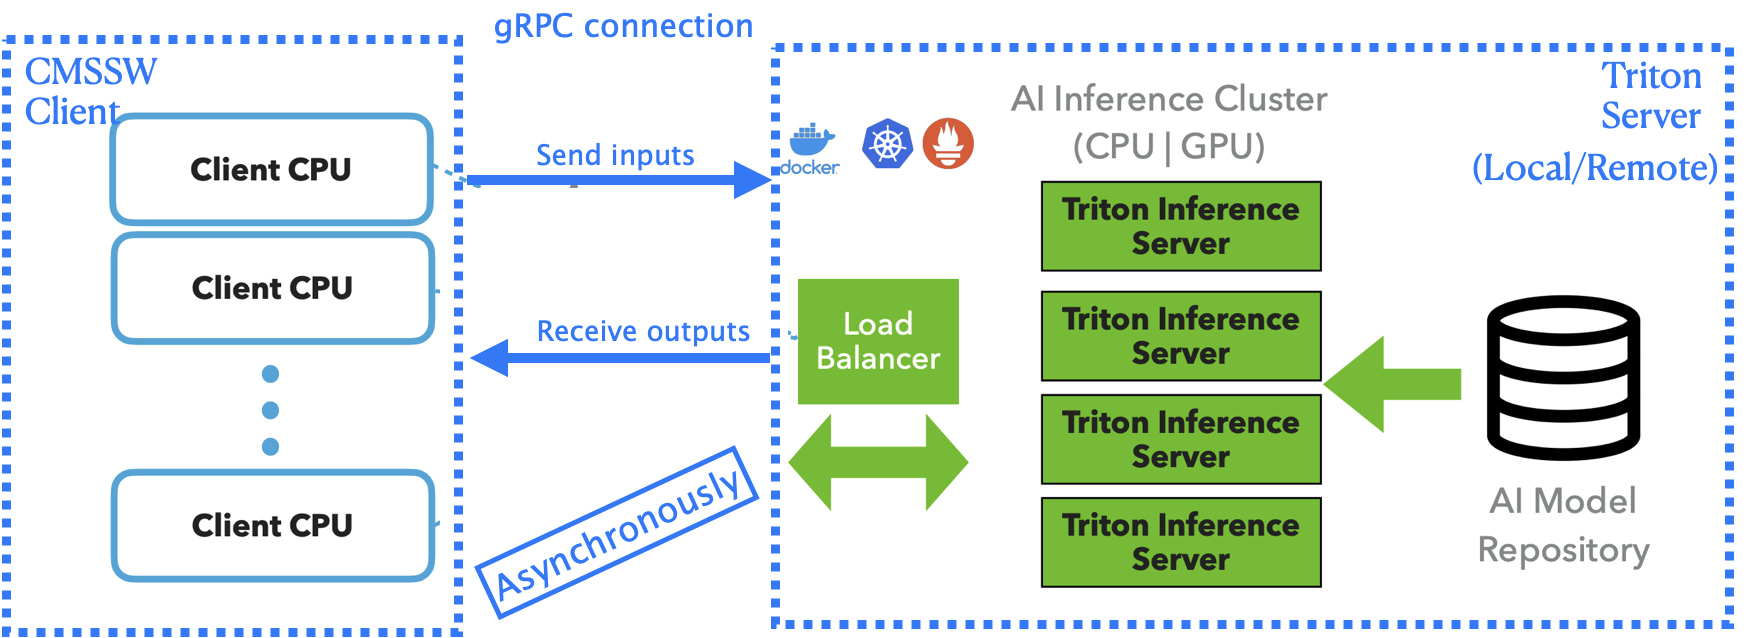
\includegraphics[width=0.90\textwidth]{plots/Architecture.png}
    \caption{Illustration of the SONIC implementation of inference as-a-service in \CMSSW. This figure also shows the possibility of an additional load-balancing layer in the SONIC scheme; for example, if multiple coprocessor-enabled machines are used to host servers, a Kubernetes engine can be set up to distribute inference calls across the machines. \textcolor{red}{(Plot will be updated to better quality)}}
    \label{fig:architecture}
\end{figure}

Within CMSSW, a mechanism has been implemented to account for the possibility that a client job cannot access a specified server for whatever reason. In this case, a ``fallback'' server is automatically created using either GPU resources if they are available or the CPU resources allocated to the client job in question. The client then makes gRPC calls to that local fallback server, which introduces negligible latency. The server overhead generally consumes very little of the CPU resources beyond what would be used for conventional inference, such that the per-event latency is not strongly affected by SONIC relative to running without SONIC. Fallback servers are automatically shut down when the job finishes. Studies related to these fallback servers are discussed in Section~\ref{sec:fallback}.

\subsection{NVIDIA Triton Inference Server}
\label{sec:triton}
%Document a brief introduction about the NVIDIA Triton inference server

As shown in Fig.~\ref{fig:architecture}, the GPU-based implementation of SONIC in \CMSSW uses the NVIDIA Triton Inference Server to deploy ML inference on the coprocessors~\cite{triton, triton_readme}. Triton servers can perform inference for ML algorithms, or ``models'', in most modern formats, including \PYTORCH, TensorRT, ONNX Runtime, \TENSORFLOW, and \XGBOOST, and also supports custom backends for alternative tasks. A single server can host multiple models at the same time or even multiple instances of the same model to allow concurrent inference requests. Triton also supports dynamic batching: if multiple inference calls are made within a window of time, the server can concatenate all calls' inputs into a single batch, which improves the GPU utilization and therefore increases the overall throughput. Parameters such as the number of model instances on a single server, the length of a batching window, and the optimal batch size are tunable and can be optimized on a case-by-case basis. Triton provides a model analyzer tool to aid in this optimization~\cite{triton_model_analyzer}.

Triton servers can use one or multiple GPUs on the same machine with a built-in load balancer. Triton servers can also run purely on CPU resources when there are no GPU resources available. For other types of coprocessors, Triton servers can also be used with the help of custom backends. To start a server, it is only necessary to provide a trained model file and sometimes a configuration file specifying input and output variable names, shapes, types, and model versions. Client-side jobs are configured with servers' address and port numbers in order to carry out communications, and jobs must provide input with the correct format for inference.

It is important to note that Triton provides an open source solution for implementing IaaS, with a public set of protocols. It is also possible to use those protocols in alternative server implementations, as was done in the FPGAs-as-a-Service Toolkit~\cite{FaaST}.%not strictly necessary to use Triton's set of protocols; for example, server protocols were independently reimplemented for communication with inference servers in the FPGAs-as-a-Service Toolkit~\cite{FaaST}.

\subsection{SONIC Discussions}
\label{sec:sonic_benefits}
\textcolor{red}{This section should also includes the discussions on the possible extra costs with SONIC: memory, network, complexity, and the compare the tradeoffs between SONIC and direct inferences.}

While many of the benefits of running with SONIC have been mentioned throughout the preceding text, it is worthwhile to quickly summarize some of these points here.
\begin{itemize}
    \item \emph{Containerization}: SONIC factorizes ML frameworks out of the client software stack, i.e., \CMSSW, making it easier support a wide variety of ML models. Currently, any ML algorithms in \CMSSW must either be cast in one of a limited number of supported frameworks, or else support for a new framework must be added. With SONIC, one can use any framework supported by Triton, including custom backends, with no modification of \CMSSW needed. This allows physicists to pick the best ML inference backend with less concern for the implementation details. This ``support'' for a wide variety of frameworks is easy to maintain.
    \item \emph{Simplicity}: Because of the containerization discussed above, client-side code that takes advantage of SONIC can be simplified. Generic functions for sending input to and receiving output from servers can be defined, and then to deploy any model deployed in the workflow, client code only needs to format model inputs correctly and collect the outputs.
    \item \emph{Flexibility}: In the SONIC paradigm, the ratio of CPU resources to GPU resources is not fixed, as clients from many different machines can access a single server running on either one GPU or multiple GPUs. Similarly, a single client can access multiple different servers running on multiple different machines. GPU-to-CPU ratios can therefore be adjusted for different ML inference tasks, allowing optimal utilization of coprocessor resources.
    \item \emph{Efficiency}: SONIC enables superior utilization of coprocessor resources. By optimizing the GPU-to-CPU ratio, it is easier to come close to saturating GPU resources without oversaturating them. Because of this, any GPU purchase can be kept to the minimal number of GPUs necessary, saving overall cost.
    \item \emph{Portability}: Through the use of SONIC, client-side workflows do not have to be modified to take advantage of different types of coprocessors. As long as a consistent protocol exists for communicating with the inference server, it does not matter if the server is on a CPU, GPU, FPGA, IPU, or any other architecture. This allows users to easily take advantage of whatever resources are available and easily optimize workflows if there are multiple options.
    \item \emph{Accessibility}: It is worth explicitly pointing out that SONIC is the only way for any CPU to access remote GPUs or other coprocessors. This should reduce costs associated with coprocessor-based inference acceleration, allowing for collaborators to share resources more easily. While calls to a remote server introduce a distance-dependent latency, the use of asynchronous calls in SONIC means that the overall event latency is negligibly impacted~\cite{Krupa:2020bwg}. SONIC can also use local resources if they are available.
\end{itemize}
